% =============================================================================
% Fig 1: DeepONet Architecture Schematic for TS Profile Fitting
% Compile standalone: pdflatex fig1_architecture.tex
% Or embed in manuscript: % =============================================================================
% Fig 1: DeepONet Architecture Schematic for TS Profile Fitting
% Compile standalone: pdflatex fig1_architecture.tex
% Or embed in manuscript: % =============================================================================
% Fig 1: DeepONet Architecture Schematic for TS Profile Fitting
% Compile standalone: pdflatex fig1_architecture.tex
% Or embed in manuscript: % =============================================================================
% Fig 1: DeepONet Architecture Schematic for TS Profile Fitting
% Compile standalone: pdflatex fig1_architecture.tex
% Or embed in manuscript: \input{fig1_architecture.tex}
% =============================================================================
\documentclass[tikz,border=5pt]{standalone}
\usepackage{amsmath,amssymb}
\usepackage{tikz}
\usetikzlibrary{positioning,shapes.geometric,arrows.meta,fit,backgrounds,decorations.pathreplacing}

\begin{document}
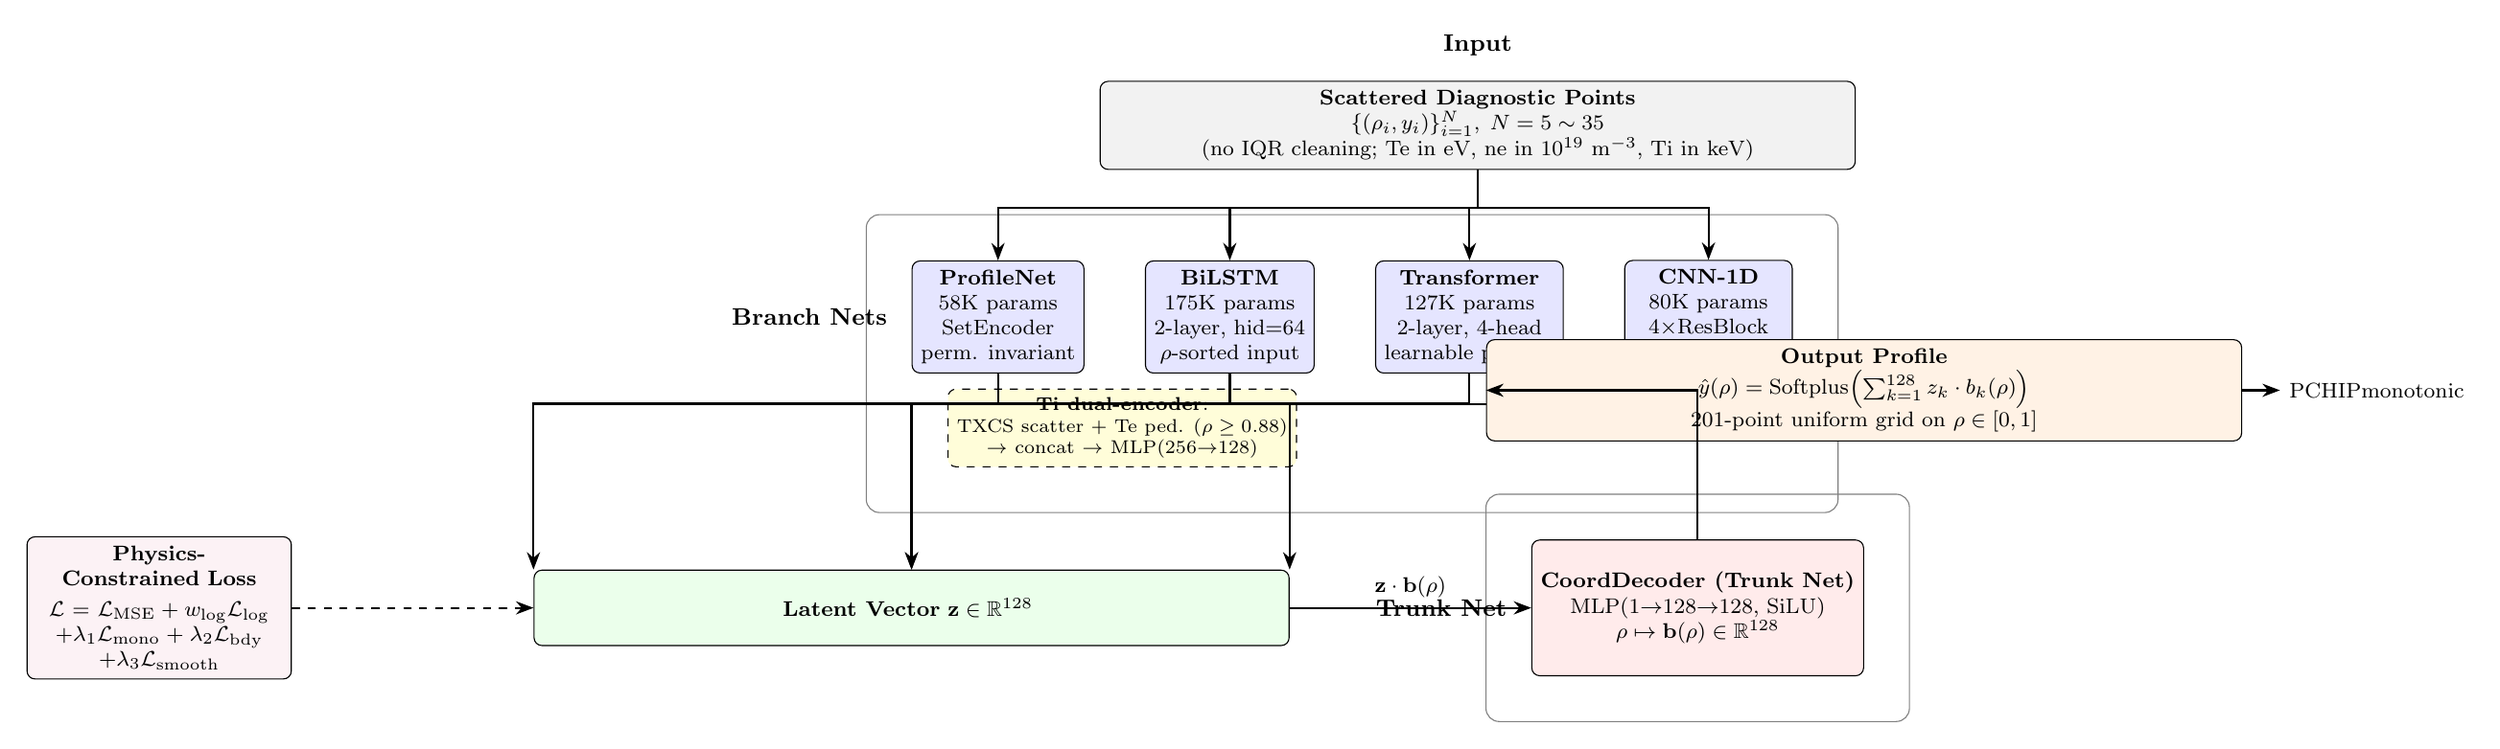
\begin{tikzpicture}[
    node distance=8mm,
    box/.style={rectangle,draw,rounded corners=3pt,align=center,minimum width=22mm,minimum height=10mm,font=\footnotesize},
    widebox/.style={box,minimum width=100mm},
    encoder/.style={box,fill=blue!10,minimum height=14mm},
    arrow/.style={-{Stealth},thick},
    label/.style={font=\footnotesize\itshape},
]

% ===== Input =====
\node[widebox,fill=gray!10] (input) {
    \textbf{Scattered Diagnostic Points}\\
    $\{(\rho_i, y_i)\}_{i=1}^N,\; N=5\sim35$\\
    {\footnotesize(no IQR cleaning; Te in eV, ne in $10^{19}$ m$^{-3}$, Ti in keV)}
};

% ===== Four Encoders (Branch Nets) =====
\node[encoder,below left=12mm and 2mm of input.south west] (profilenet) {
    \textbf{ProfileNet}\\
    58K params\\
    {\footnotesize SetEncoder}\\
    {\footnotesize perm. invariant}
};
\node[encoder,right=of profilenet] (lstm) {
    \textbf{BiLSTM}\\
    175K params\\
    {\footnotesize 2-layer, hid=64}\\
    {\footnotesize $\rho$-sorted input}
};
\node[encoder,right=of lstm] (transformer) {
    \textbf{Transformer}\\
    127K params\\
    {\footnotesize 2-layer, 4-head}\\
    {\footnotesize learnable pos-enc}
};
\node[encoder,right=of transformer] (cnn) {
    \textbf{CNN-1D}\\
    80K params\\
    {\footnotesize 4$\times$ResBlock}\\
    {\footnotesize (control group)}
};

% Connect input to encoders using coordinate trick
\coordinate (in_bottom) at (input.south);
\draw[arrow] (in_bottom) -- ++(0,-5mm) -| (profilenet.north);
\draw[arrow] (in_bottom) -- ++(0,-5mm) -| (lstm.north);
\draw[arrow] (in_bottom) -- ++(0,-5mm) -| (transformer.north);
\draw[arrow] (in_bottom) -- ++(0,-5mm) -| (cnn.north);

% ===== Ti Dual Encoder annotation =====
\node[box,fill=yellow!15,dashed,below=2mm of profilenet.south east,xshift=5mm,font=\scriptsize] (tidual) {
    \textbf{Ti dual-encoder}:\\
    TXCS scatter + Te ped. ($\rho\geq 0.88$)\\
    $\to$ concat $\to$ MLP(256$\to$128)
};

% ===== Latent Vector =====
\node[widebox,fill=green!8,below=16mm of profilenet.south west,yshift=-10mm] (z) {
    \textbf{Latent Vector} $\mathbf{z}\in\mathbb{R}^{128}$
};

% Encoder outputs to z
\draw[arrow] (profilenet.south) -- ++(0,-4mm) -| (z.north west);
\draw[arrow] (lstm.south) -- ++(0,-4mm) -| (z.north);
\draw[arrow] (transformer.south) -- ++(0,-4mm) -| (z.north);
\draw[arrow] (cnn.south) -- ++(0,-4mm) -| (z.north east);

% ===== CoordDecoder (Trunk Net) =====
\node[box,fill=red!8,right=32mm of z.east,minimum width=38mm,minimum height=18mm] (coorddecoder) {
    \textbf{CoordDecoder (Trunk Net)}\\
    MLP(1$\to$128$\to$128, SiLU)\\
    $\rho \mapsto \mathbf{b}(\rho)\in\mathbb{R}^{128}$
};

% ===== Output =====
\node[widebox,fill=orange!10,above=of coorddecoder.north east,yshift=5mm] (output) {
    \textbf{Output Profile}\\
    $\hat{y}(\rho) = \mathrm{Softplus}\!\left(\sum_{k=1}^{128} z_k\cdot b_k(\rho)\right)$\\
    {\footnotesize 201-point uniform grid on $\rho\in[0,1]$}
};

% Connections
\draw[arrow] (z.east) -- node[label,above] {$\mathbf{z}\cdot\mathbf{b}(\rho)$} (coorddecoder.west);
\draw[arrow] (coorddecoder.north) |- (output.west);

% PCHIP post-processing arrow
\node[right=5mm of output.east,font=\footnotesize] (pchip) {PCHIP\\monotonic};
\draw[arrow] (output.east) -- (pchip.west);

% ===== Loss Function box (left side) =====
\node[box,fill=purple!5,left=32mm of z.west,minimum width=35mm,text width=32mm,font=\footnotesize] (loss) {
    \textbf{Physics-Constrained Loss}\\[2pt]
    $\mathcal{L} = \mathcal{L}_{\text{MSE}} + w_{\log}\mathcal{L}_{\log}$\\
    $+ \lambda_1\mathcal{L}_{\text{mono}} + \lambda_2\mathcal{L}_{\text{bdy}}$\\
    $+ \lambda_3\mathcal{L}_{\text{smooth}}$
};
\draw[arrow,dashed] (loss.east) -- (z.west);

% ===== Labels =====
\node[font=\small\bfseries,above=2mm of input.north] {Input};
\node[font=\small\bfseries,left=2mm of profilenet.west] {Branch Nets};
\node[font=\small\bfseries,left=2mm of coorddecoder.west] {Trunk Net};

% ===== Group boxes =====
\begin{scope}[on background layer]
    \node[draw=gray,inner sep=6mm,rounded corners=5pt,fit=(profilenet)(cnn)(tidual),label={[anchor=north west]north west:\textbf{Encoder (4 variants)}}] {};
    \node[draw=gray,inner sep=6mm,rounded corners=5pt,fit=(coorddecoder),label={[anchor=north west]north west:\textbf{Decoder (shared)}}] {};
\end{scope}

\end{tikzpicture}
\end{document}

% =============================================================================
\documentclass[tikz,border=5pt]{standalone}
\usepackage{amsmath,amssymb}
\usepackage{tikz}
\usetikzlibrary{positioning,shapes.geometric,arrows.meta,fit,backgrounds,decorations.pathreplacing}

\begin{document}
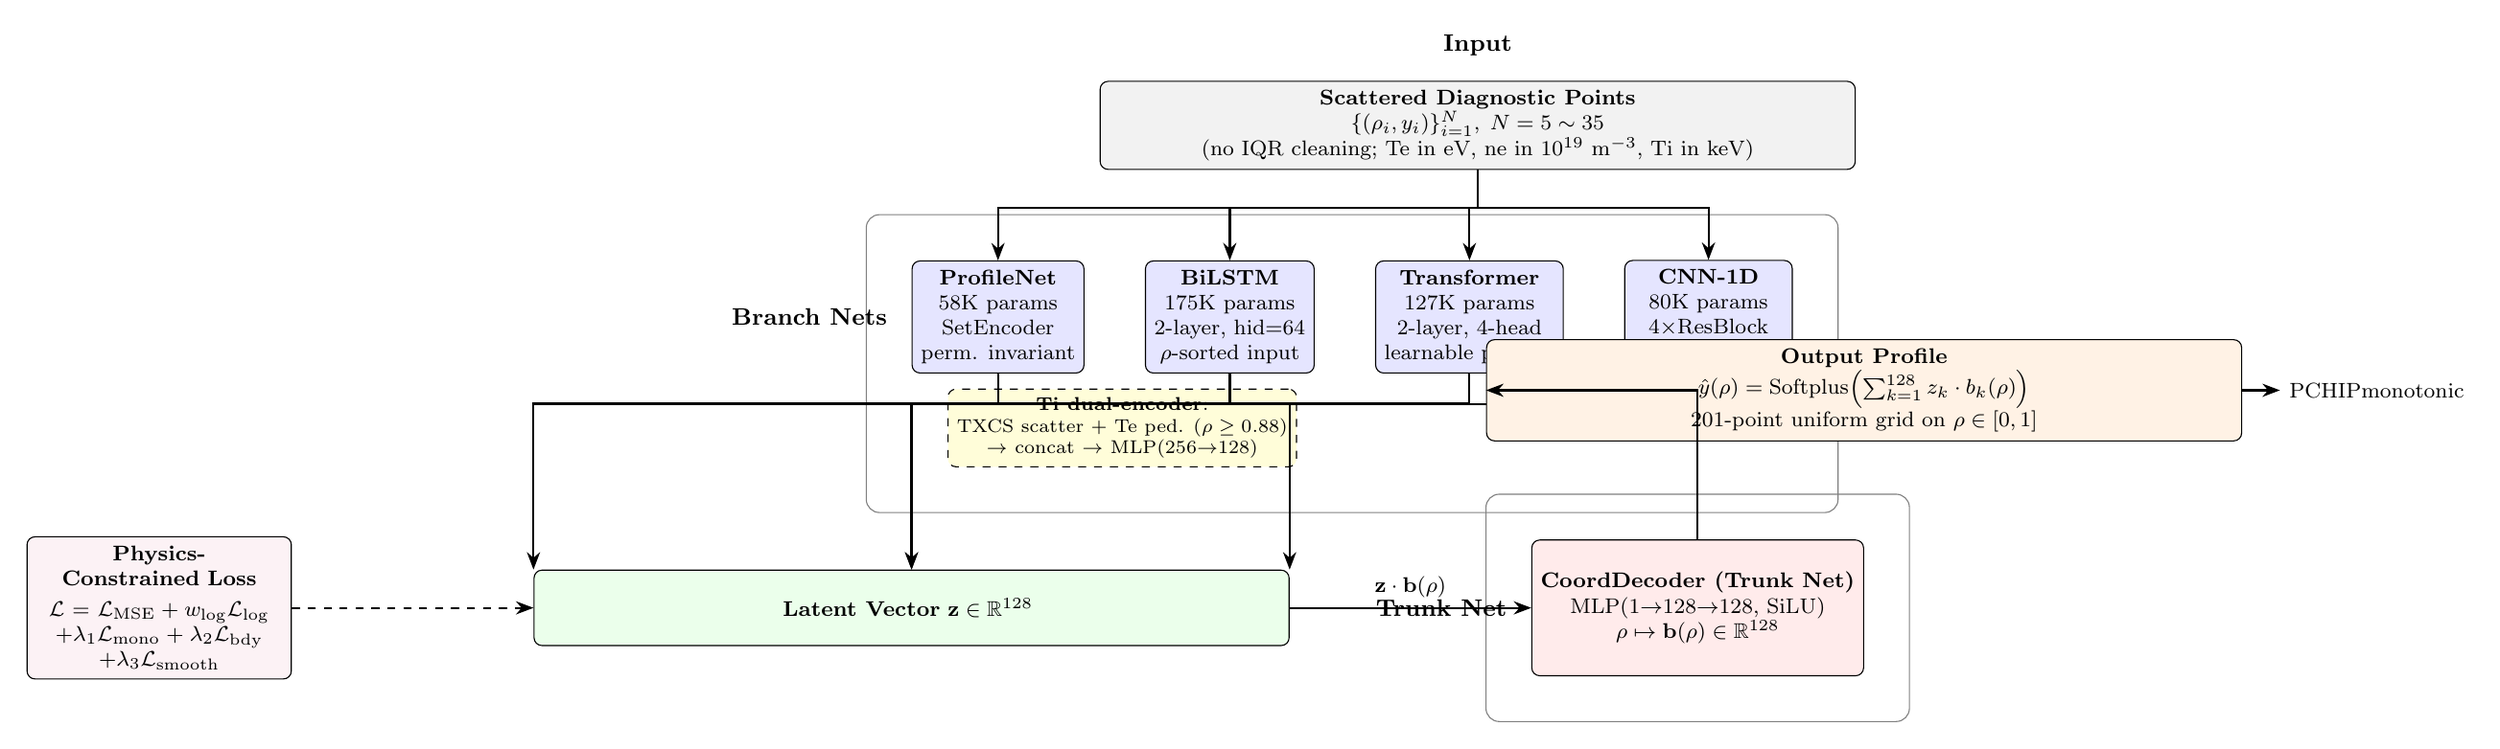
\begin{tikzpicture}[
    node distance=8mm,
    box/.style={rectangle,draw,rounded corners=3pt,align=center,minimum width=22mm,minimum height=10mm,font=\footnotesize},
    widebox/.style={box,minimum width=100mm},
    encoder/.style={box,fill=blue!10,minimum height=14mm},
    arrow/.style={-{Stealth},thick},
    label/.style={font=\footnotesize\itshape},
]

% ===== Input =====
\node[widebox,fill=gray!10] (input) {
    \textbf{Scattered Diagnostic Points}\\
    $\{(\rho_i, y_i)\}_{i=1}^N,\; N=5\sim35$\\
    {\footnotesize(no IQR cleaning; Te in eV, ne in $10^{19}$ m$^{-3}$, Ti in keV)}
};

% ===== Four Encoders (Branch Nets) =====
\node[encoder,below left=12mm and 2mm of input.south west] (profilenet) {
    \textbf{ProfileNet}\\
    58K params\\
    {\footnotesize SetEncoder}\\
    {\footnotesize perm. invariant}
};
\node[encoder,right=of profilenet] (lstm) {
    \textbf{BiLSTM}\\
    175K params\\
    {\footnotesize 2-layer, hid=64}\\
    {\footnotesize $\rho$-sorted input}
};
\node[encoder,right=of lstm] (transformer) {
    \textbf{Transformer}\\
    127K params\\
    {\footnotesize 2-layer, 4-head}\\
    {\footnotesize learnable pos-enc}
};
\node[encoder,right=of transformer] (cnn) {
    \textbf{CNN-1D}\\
    80K params\\
    {\footnotesize 4$\times$ResBlock}\\
    {\footnotesize (control group)}
};

% Connect input to encoders using coordinate trick
\coordinate (in_bottom) at (input.south);
\draw[arrow] (in_bottom) -- ++(0,-5mm) -| (profilenet.north);
\draw[arrow] (in_bottom) -- ++(0,-5mm) -| (lstm.north);
\draw[arrow] (in_bottom) -- ++(0,-5mm) -| (transformer.north);
\draw[arrow] (in_bottom) -- ++(0,-5mm) -| (cnn.north);

% ===== Ti Dual Encoder annotation =====
\node[box,fill=yellow!15,dashed,below=2mm of profilenet.south east,xshift=5mm,font=\scriptsize] (tidual) {
    \textbf{Ti dual-encoder}:\\
    TXCS scatter + Te ped. ($\rho\geq 0.88$)\\
    $\to$ concat $\to$ MLP(256$\to$128)
};

% ===== Latent Vector =====
\node[widebox,fill=green!8,below=16mm of profilenet.south west,yshift=-10mm] (z) {
    \textbf{Latent Vector} $\mathbf{z}\in\mathbb{R}^{128}$
};

% Encoder outputs to z
\draw[arrow] (profilenet.south) -- ++(0,-4mm) -| (z.north west);
\draw[arrow] (lstm.south) -- ++(0,-4mm) -| (z.north);
\draw[arrow] (transformer.south) -- ++(0,-4mm) -| (z.north);
\draw[arrow] (cnn.south) -- ++(0,-4mm) -| (z.north east);

% ===== CoordDecoder (Trunk Net) =====
\node[box,fill=red!8,right=32mm of z.east,minimum width=38mm,minimum height=18mm] (coorddecoder) {
    \textbf{CoordDecoder (Trunk Net)}\\
    MLP(1$\to$128$\to$128, SiLU)\\
    $\rho \mapsto \mathbf{b}(\rho)\in\mathbb{R}^{128}$
};

% ===== Output =====
\node[widebox,fill=orange!10,above=of coorddecoder.north east,yshift=5mm] (output) {
    \textbf{Output Profile}\\
    $\hat{y}(\rho) = \mathrm{Softplus}\!\left(\sum_{k=1}^{128} z_k\cdot b_k(\rho)\right)$\\
    {\footnotesize 201-point uniform grid on $\rho\in[0,1]$}
};

% Connections
\draw[arrow] (z.east) -- node[label,above] {$\mathbf{z}\cdot\mathbf{b}(\rho)$} (coorddecoder.west);
\draw[arrow] (coorddecoder.north) |- (output.west);

% PCHIP post-processing arrow
\node[right=5mm of output.east,font=\footnotesize] (pchip) {PCHIP\\monotonic};
\draw[arrow] (output.east) -- (pchip.west);

% ===== Loss Function box (left side) =====
\node[box,fill=purple!5,left=32mm of z.west,minimum width=35mm,text width=32mm,font=\footnotesize] (loss) {
    \textbf{Physics-Constrained Loss}\\[2pt]
    $\mathcal{L} = \mathcal{L}_{\text{MSE}} + w_{\log}\mathcal{L}_{\log}$\\
    $+ \lambda_1\mathcal{L}_{\text{mono}} + \lambda_2\mathcal{L}_{\text{bdy}}$\\
    $+ \lambda_3\mathcal{L}_{\text{smooth}}$
};
\draw[arrow,dashed] (loss.east) -- (z.west);

% ===== Labels =====
\node[font=\small\bfseries,above=2mm of input.north] {Input};
\node[font=\small\bfseries,left=2mm of profilenet.west] {Branch Nets};
\node[font=\small\bfseries,left=2mm of coorddecoder.west] {Trunk Net};

% ===== Group boxes =====
\begin{scope}[on background layer]
    \node[draw=gray,inner sep=6mm,rounded corners=5pt,fit=(profilenet)(cnn)(tidual),label={[anchor=north west]north west:\textbf{Encoder (4 variants)}}] {};
    \node[draw=gray,inner sep=6mm,rounded corners=5pt,fit=(coorddecoder),label={[anchor=north west]north west:\textbf{Decoder (shared)}}] {};
\end{scope}

\end{tikzpicture}
\end{document}

% =============================================================================
\documentclass[tikz,border=5pt]{standalone}
\usepackage{amsmath,amssymb}
\usepackage{tikz}
\usetikzlibrary{positioning,shapes.geometric,arrows.meta,fit,backgrounds,decorations.pathreplacing}

\begin{document}
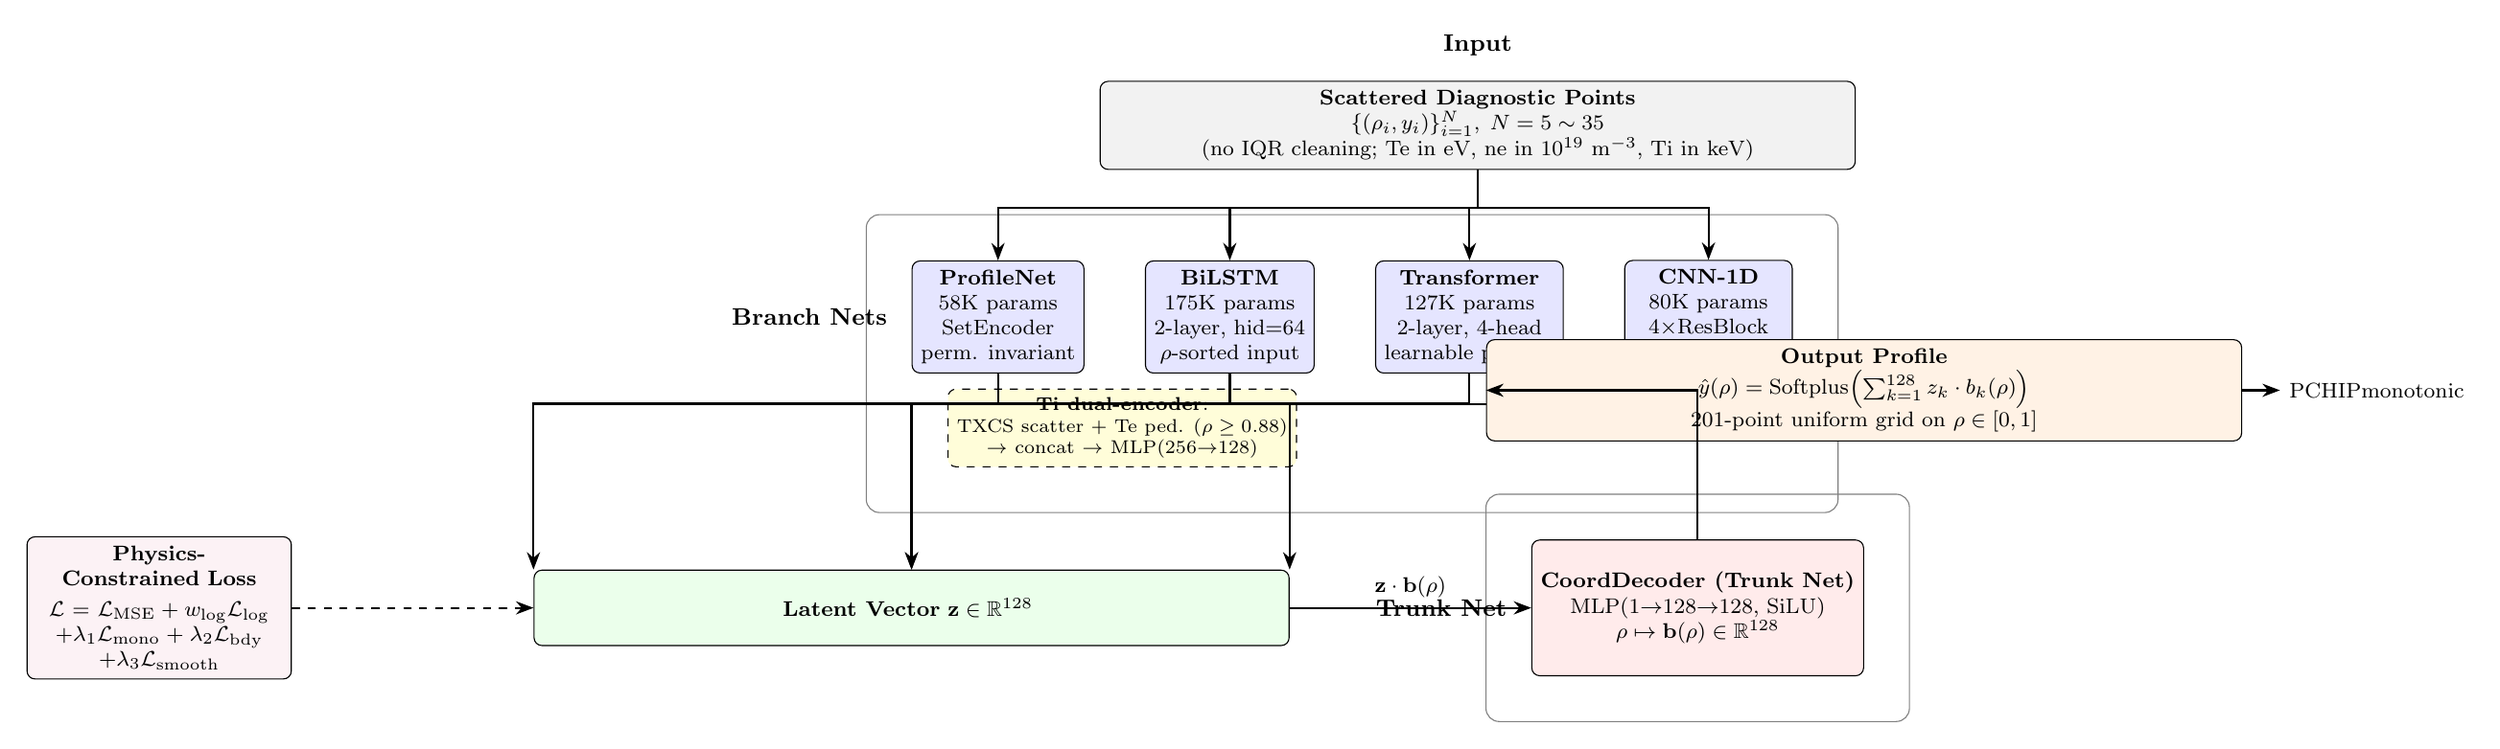
\begin{tikzpicture}[
    node distance=8mm,
    box/.style={rectangle,draw,rounded corners=3pt,align=center,minimum width=22mm,minimum height=10mm,font=\footnotesize},
    widebox/.style={box,minimum width=100mm},
    encoder/.style={box,fill=blue!10,minimum height=14mm},
    arrow/.style={-{Stealth},thick},
    label/.style={font=\footnotesize\itshape},
]

% ===== Input =====
\node[widebox,fill=gray!10] (input) {
    \textbf{Scattered Diagnostic Points}\\
    $\{(\rho_i, y_i)\}_{i=1}^N,\; N=5\sim35$\\
    {\footnotesize(no IQR cleaning; Te in eV, ne in $10^{19}$ m$^{-3}$, Ti in keV)}
};

% ===== Four Encoders (Branch Nets) =====
\node[encoder,below left=12mm and 2mm of input.south west] (profilenet) {
    \textbf{ProfileNet}\\
    58K params\\
    {\footnotesize SetEncoder}\\
    {\footnotesize perm. invariant}
};
\node[encoder,right=of profilenet] (lstm) {
    \textbf{BiLSTM}\\
    175K params\\
    {\footnotesize 2-layer, hid=64}\\
    {\footnotesize $\rho$-sorted input}
};
\node[encoder,right=of lstm] (transformer) {
    \textbf{Transformer}\\
    127K params\\
    {\footnotesize 2-layer, 4-head}\\
    {\footnotesize learnable pos-enc}
};
\node[encoder,right=of transformer] (cnn) {
    \textbf{CNN-1D}\\
    80K params\\
    {\footnotesize 4$\times$ResBlock}\\
    {\footnotesize (control group)}
};

% Connect input to encoders using coordinate trick
\coordinate (in_bottom) at (input.south);
\draw[arrow] (in_bottom) -- ++(0,-5mm) -| (profilenet.north);
\draw[arrow] (in_bottom) -- ++(0,-5mm) -| (lstm.north);
\draw[arrow] (in_bottom) -- ++(0,-5mm) -| (transformer.north);
\draw[arrow] (in_bottom) -- ++(0,-5mm) -| (cnn.north);

% ===== Ti Dual Encoder annotation =====
\node[box,fill=yellow!15,dashed,below=2mm of profilenet.south east,xshift=5mm,font=\scriptsize] (tidual) {
    \textbf{Ti dual-encoder}:\\
    TXCS scatter + Te ped. ($\rho\geq 0.88$)\\
    $\to$ concat $\to$ MLP(256$\to$128)
};

% ===== Latent Vector =====
\node[widebox,fill=green!8,below=16mm of profilenet.south west,yshift=-10mm] (z) {
    \textbf{Latent Vector} $\mathbf{z}\in\mathbb{R}^{128}$
};

% Encoder outputs to z
\draw[arrow] (profilenet.south) -- ++(0,-4mm) -| (z.north west);
\draw[arrow] (lstm.south) -- ++(0,-4mm) -| (z.north);
\draw[arrow] (transformer.south) -- ++(0,-4mm) -| (z.north);
\draw[arrow] (cnn.south) -- ++(0,-4mm) -| (z.north east);

% ===== CoordDecoder (Trunk Net) =====
\node[box,fill=red!8,right=32mm of z.east,minimum width=38mm,minimum height=18mm] (coorddecoder) {
    \textbf{CoordDecoder (Trunk Net)}\\
    MLP(1$\to$128$\to$128, SiLU)\\
    $\rho \mapsto \mathbf{b}(\rho)\in\mathbb{R}^{128}$
};

% ===== Output =====
\node[widebox,fill=orange!10,above=of coorddecoder.north east,yshift=5mm] (output) {
    \textbf{Output Profile}\\
    $\hat{y}(\rho) = \mathrm{Softplus}\!\left(\sum_{k=1}^{128} z_k\cdot b_k(\rho)\right)$\\
    {\footnotesize 201-point uniform grid on $\rho\in[0,1]$}
};

% Connections
\draw[arrow] (z.east) -- node[label,above] {$\mathbf{z}\cdot\mathbf{b}(\rho)$} (coorddecoder.west);
\draw[arrow] (coorddecoder.north) |- (output.west);

% PCHIP post-processing arrow
\node[right=5mm of output.east,font=\footnotesize] (pchip) {PCHIP\\monotonic};
\draw[arrow] (output.east) -- (pchip.west);

% ===== Loss Function box (left side) =====
\node[box,fill=purple!5,left=32mm of z.west,minimum width=35mm,text width=32mm,font=\footnotesize] (loss) {
    \textbf{Physics-Constrained Loss}\\[2pt]
    $\mathcal{L} = \mathcal{L}_{\text{MSE}} + w_{\log}\mathcal{L}_{\log}$\\
    $+ \lambda_1\mathcal{L}_{\text{mono}} + \lambda_2\mathcal{L}_{\text{bdy}}$\\
    $+ \lambda_3\mathcal{L}_{\text{smooth}}$
};
\draw[arrow,dashed] (loss.east) -- (z.west);

% ===== Labels =====
\node[font=\small\bfseries,above=2mm of input.north] {Input};
\node[font=\small\bfseries,left=2mm of profilenet.west] {Branch Nets};
\node[font=\small\bfseries,left=2mm of coorddecoder.west] {Trunk Net};

% ===== Group boxes =====
\begin{scope}[on background layer]
    \node[draw=gray,inner sep=6mm,rounded corners=5pt,fit=(profilenet)(cnn)(tidual),label={[anchor=north west]north west:\textbf{Encoder (4 variants)}}] {};
    \node[draw=gray,inner sep=6mm,rounded corners=5pt,fit=(coorddecoder),label={[anchor=north west]north west:\textbf{Decoder (shared)}}] {};
\end{scope}

\end{tikzpicture}
\end{document}

% =============================================================================
\documentclass[tikz,border=5pt]{standalone}
\usepackage{amsmath,amssymb}
\usepackage{tikz}
\usetikzlibrary{positioning,shapes.geometric,arrows.meta,fit,backgrounds,decorations.pathreplacing}

\begin{document}
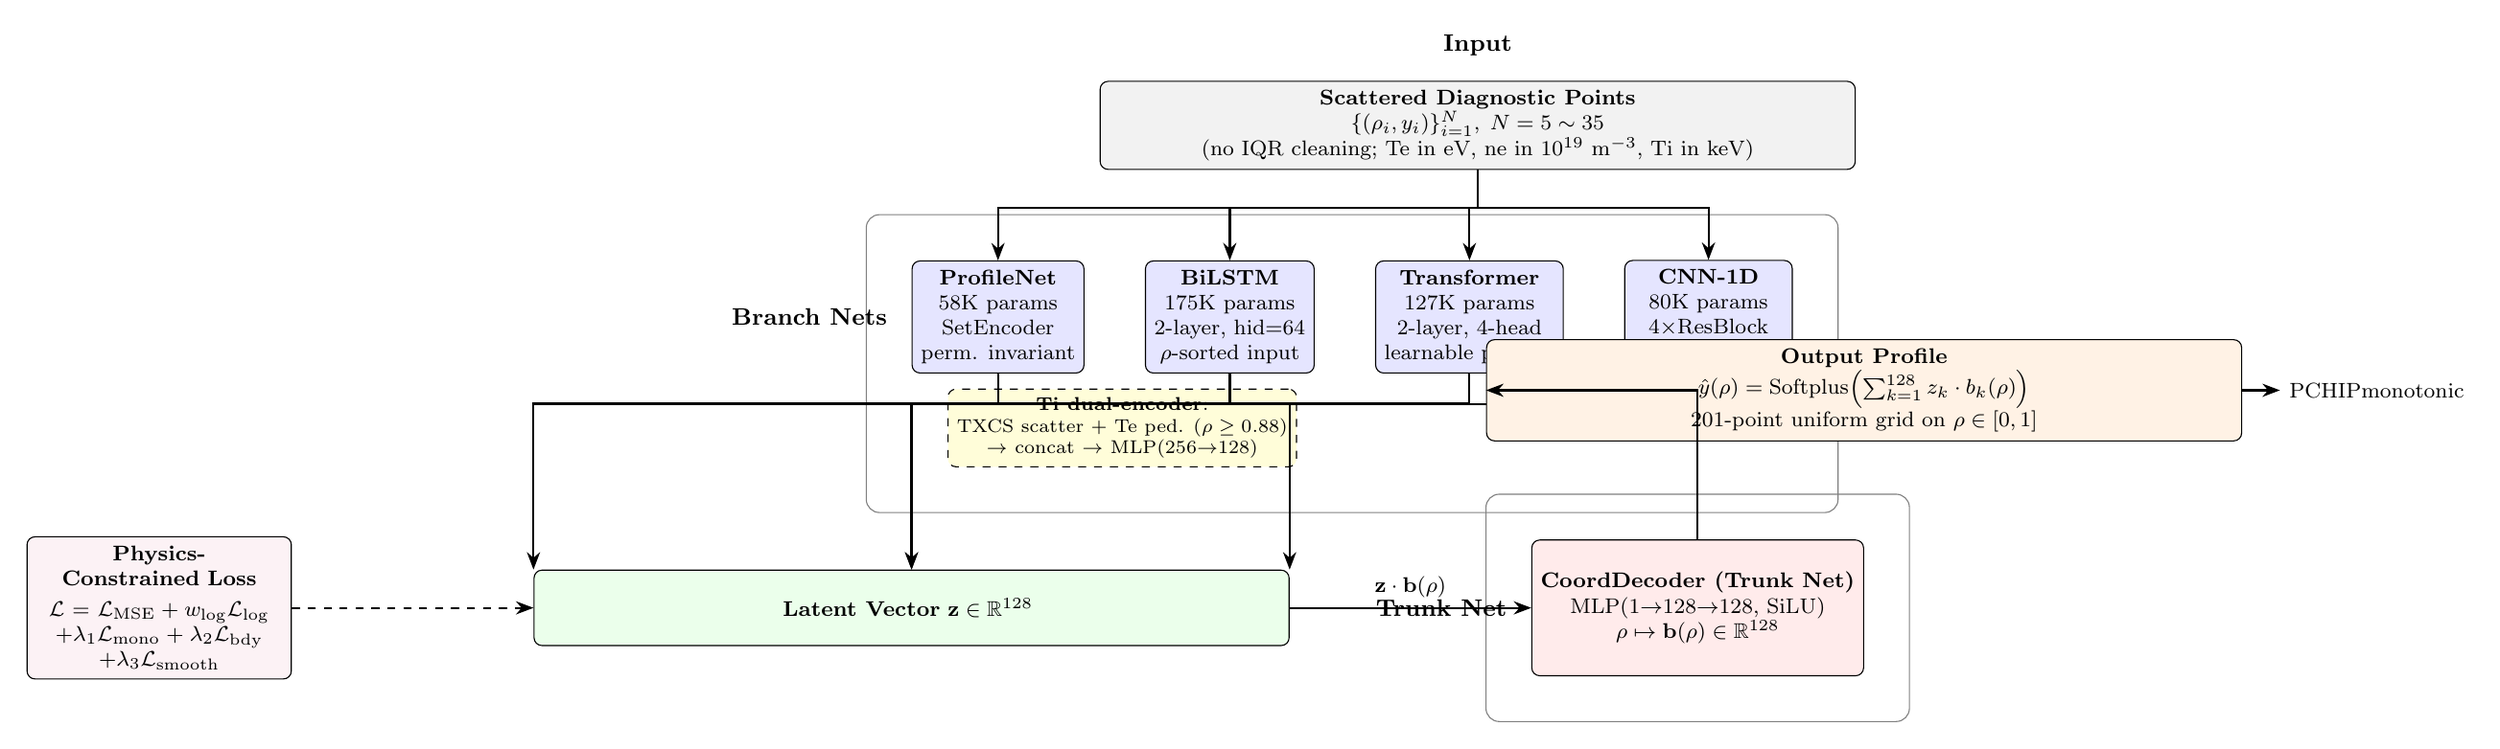
\begin{tikzpicture}[
    node distance=8mm,
    box/.style={rectangle,draw,rounded corners=3pt,align=center,minimum width=22mm,minimum height=10mm,font=\footnotesize},
    widebox/.style={box,minimum width=100mm},
    encoder/.style={box,fill=blue!10,minimum height=14mm},
    arrow/.style={-{Stealth},thick},
    label/.style={font=\footnotesize\itshape},
]

% ===== Input =====
\node[widebox,fill=gray!10] (input) {
    \textbf{Scattered Diagnostic Points}\\
    $\{(\rho_i, y_i)\}_{i=1}^N,\; N=5\sim35$\\
    {\footnotesize(no IQR cleaning; Te in eV, ne in $10^{19}$ m$^{-3}$, Ti in keV)}
};

% ===== Four Encoders (Branch Nets) =====
\node[encoder,below left=12mm and 2mm of input.south west] (profilenet) {
    \textbf{ProfileNet}\\
    58K params\\
    {\footnotesize SetEncoder}\\
    {\footnotesize perm. invariant}
};
\node[encoder,right=of profilenet] (lstm) {
    \textbf{BiLSTM}\\
    175K params\\
    {\footnotesize 2-layer, hid=64}\\
    {\footnotesize $\rho$-sorted input}
};
\node[encoder,right=of lstm] (transformer) {
    \textbf{Transformer}\\
    127K params\\
    {\footnotesize 2-layer, 4-head}\\
    {\footnotesize learnable pos-enc}
};
\node[encoder,right=of transformer] (cnn) {
    \textbf{CNN-1D}\\
    80K params\\
    {\footnotesize 4$\times$ResBlock}\\
    {\footnotesize (control group)}
};

% Connect input to encoders using coordinate trick
\coordinate (in_bottom) at (input.south);
\draw[arrow] (in_bottom) -- ++(0,-5mm) -| (profilenet.north);
\draw[arrow] (in_bottom) -- ++(0,-5mm) -| (lstm.north);
\draw[arrow] (in_bottom) -- ++(0,-5mm) -| (transformer.north);
\draw[arrow] (in_bottom) -- ++(0,-5mm) -| (cnn.north);

% ===== Ti Dual Encoder annotation =====
\node[box,fill=yellow!15,dashed,below=2mm of profilenet.south east,xshift=5mm,font=\scriptsize] (tidual) {
    \textbf{Ti dual-encoder}:\\
    TXCS scatter + Te ped. ($\rho\geq 0.88$)\\
    $\to$ concat $\to$ MLP(256$\to$128)
};

% ===== Latent Vector =====
\node[widebox,fill=green!8,below=16mm of profilenet.south west,yshift=-10mm] (z) {
    \textbf{Latent Vector} $\mathbf{z}\in\mathbb{R}^{128}$
};

% Encoder outputs to z
\draw[arrow] (profilenet.south) -- ++(0,-4mm) -| (z.north west);
\draw[arrow] (lstm.south) -- ++(0,-4mm) -| (z.north);
\draw[arrow] (transformer.south) -- ++(0,-4mm) -| (z.north);
\draw[arrow] (cnn.south) -- ++(0,-4mm) -| (z.north east);

% ===== CoordDecoder (Trunk Net) =====
\node[box,fill=red!8,right=32mm of z.east,minimum width=38mm,minimum height=18mm] (coorddecoder) {
    \textbf{CoordDecoder (Trunk Net)}\\
    MLP(1$\to$128$\to$128, SiLU)\\
    $\rho \mapsto \mathbf{b}(\rho)\in\mathbb{R}^{128}$
};

% ===== Output =====
\node[widebox,fill=orange!10,above=of coorddecoder.north east,yshift=5mm] (output) {
    \textbf{Output Profile}\\
    $\hat{y}(\rho) = \mathrm{Softplus}\!\left(\sum_{k=1}^{128} z_k\cdot b_k(\rho)\right)$\\
    {\footnotesize 201-point uniform grid on $\rho\in[0,1]$}
};

% Connections
\draw[arrow] (z.east) -- node[label,above] {$\mathbf{z}\cdot\mathbf{b}(\rho)$} (coorddecoder.west);
\draw[arrow] (coorddecoder.north) |- (output.west);

% PCHIP post-processing arrow
\node[right=5mm of output.east,font=\footnotesize] (pchip) {PCHIP\\monotonic};
\draw[arrow] (output.east) -- (pchip.west);

% ===== Loss Function box (left side) =====
\node[box,fill=purple!5,left=32mm of z.west,minimum width=35mm,text width=32mm,font=\footnotesize] (loss) {
    \textbf{Physics-Constrained Loss}\\[2pt]
    $\mathcal{L} = \mathcal{L}_{\text{MSE}} + w_{\log}\mathcal{L}_{\log}$\\
    $+ \lambda_1\mathcal{L}_{\text{mono}} + \lambda_2\mathcal{L}_{\text{bdy}}$\\
    $+ \lambda_3\mathcal{L}_{\text{smooth}}$
};
\draw[arrow,dashed] (loss.east) -- (z.west);

% ===== Labels =====
\node[font=\small\bfseries,above=2mm of input.north] {Input};
\node[font=\small\bfseries,left=2mm of profilenet.west] {Branch Nets};
\node[font=\small\bfseries,left=2mm of coorddecoder.west] {Trunk Net};

% ===== Group boxes =====
\begin{scope}[on background layer]
    \node[draw=gray,inner sep=6mm,rounded corners=5pt,fit=(profilenet)(cnn)(tidual),label={[anchor=north west]north west:\textbf{Encoder (4 variants)}}] {};
    \node[draw=gray,inner sep=6mm,rounded corners=5pt,fit=(coorddecoder),label={[anchor=north west]north west:\textbf{Decoder (shared)}}] {};
\end{scope}

\end{tikzpicture}
\end{document}
